\newcommand{\CostCurveFigure}{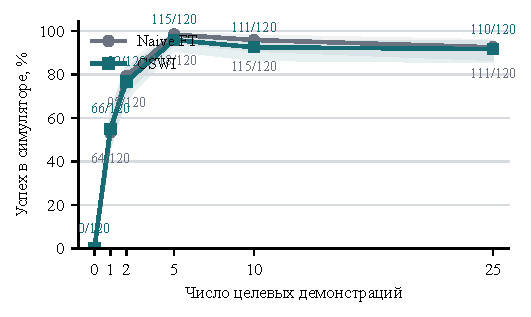
\includegraphics[width=\linewidth]{report/cost_curve.pdf}}
\newcommand{\MainResultTable}{%
\begin{tabular}{lrrrrrr}\toprule
метод & 0 & 1 & 2 & 5 & 10 & 25\\\midrule
Naive FT & 0.0 [0.0; 3.1] & 53.3 [44.4; 62.0] & 79.2 [71.1; 85.5] & 98.3 [94.1; 99.5] & 95.8 [90.6; 98.2] & 92.5 [86.4; 96.0]\\
CSWI & 0.0 [0.0; 3.1] & 55.0 [46.1; 63.6] & 76.7 [68.3; 83.3] & 95.8 [90.6; 98.2] & 92.5 [86.4; 96.0] & 91.7 [85.3; 95.4]\\
\bottomrule
\end{tabular}
}
\newcommand{\PerTaskTable}{%
\begin{tabular}{lrrrrr}\toprule
задача & 1 & 2 & 5 & 10 & 25\\\midrule
T0 & 0.0$\to$0.0 & 82.5$\to$75.0 & 100.0$\to$92.5 & 97.5$\to$92.5 & 95.0$\to$95.0\\
T1 & 100.0$\to$97.5 & 100.0$\to$97.5 & 100.0$\to$100.0 & 100.0$\to$97.5 & 90.0$\to$90.0\\
T2 & 60.0$\to$67.5 & 55.0$\to$57.5 & 95.0$\to$95.0 & 90.0$\to$87.5 & 92.5$\to$90.0\\
\bottomrule
\end{tabular}
}
\newcommand{\TaskDecompositionText}{%
В 15 task--budget ячейках $k=1/2/5/10/25$ положительных сдвигов 2, ничьих 5, отрицательных 8. Максимум: T2/$k=1$ (+7.5~п.п.); минимум: T0/$k=2$ (-7.5~п.п.).
}
\newcommand{\LanguageText}{%
Correct prompt: 0/120 (0.0\%); cyclic-wrong prompt: 0/120 (0.0\%); наблюдаемое падение 0.0~п.п.
}
\newcommand{\ComparisonText}{%
Парное сравнение на одинаковых initial states (двусторонний exact McNemar): $k=1$: $\Delta=+1.7$~п.п., $W/L=8/6$, exact $p=0.791$; $k=2$: $\Delta=-2.5$~п.п., $W/L=10/13$, exact $p=0.678$; $k=5$: $\Delta=-2.5$~п.п., $W/L=1/4$, exact $p=0.375$; $k=10$: $\Delta=-3.3$~п.п., $W/L=3/7$, exact $p=0.344$; $k=25$: $\Delta=-0.8$~п.п., $W/L=7/8$, exact $p=1.000$.
}
\newcommand{\PairedTable}{%
\begin{tabular}{rrrrr}\toprule
$k$ & $\Delta$, п.п. & wins & losses & exact $p$\\\midrule
1 & +1.7 & 8 & 6 & 0.791\\
2 & -2.5 & 10 & 13 & 0.678\\
5 & -2.5 & 1 & 4 & 0.375\\
10 & -3.3 & 3 & 7 & 0.344\\
25 & -0.8 & 7 & 8 & 1.000\\
\bottomrule
\end{tabular}
}
\newcommand{\RobustnessTable}{%
\begin{tabular}{lrrrr}\toprule
метод & eval seed & $\Delta_5$ & $\Delta_{10}$ & $\Delta_{25}$\\\midrule
CSWI & 1000 & +5.8 & +0.0 & +2.5\\
CSTVI & 2000 & +0.8 & +5.0 & -4.2\\
BDAM & 3000 & -4.2 & -2.5 & -2.5\\
\bottomrule
\end{tabular}
}
\newcommand{\BonusText}{%
По 42 checkpoint cells Spearman $\rho$ малого критика равен -0.323 при span score 0.0013; Robometer --- 0.252 при span 0.298. Малый критик практически коллапсировал к константе, тогда как Robometer отделяет zero-shot floor, но его положительное ранжирование остаётся умеренным и не означает калибровку reward.
}
\newcommand{\OptimizationText}{%
При прямом argmax proxy среди четырех policy на каждой из 9 task--budget групп baseline-reference равен 93.3\%. Малый критик выбирает 85.9\% ($\Delta=-7.4$~п.п.; 5/9 suboptimal), Robometer --- 91.1\% ($\Delta=-2.2$~п.п.). Следовательно, максимизация малого video-reward выбирает объективно худшую policy; Robometer устойчивее, но также не достигает simulator oracle.
}
\newcommand{\CeilingSummary}{%
На независимом eval seed 4000 для $k=1/2/5/10/25$ baseline дал [64/95/118/115/111]/120 успехов, CSWI --- [66/92/115/111/110]/120; парные изменения равны [+1.7/-2.5/-2.5/-3.3/-0.8]~п.п.
}
\newcommand{\CeilingVerdict}{%
Строгий критерий превосходства на каждом бюджете не выполнен: $k=2$, $k=5$, $k=10$, $k=25$ не дают положительного приращения.
}
\newcommand{\HypothesisFourText}{%
подтверждено: $\rho_{small}=-0.323$, $\rho_{Robo}=0.252$
}
